% This is a simple sample document.  For more complicated documents take a look in the exercise tab. Note that everything that comes after a % symbol is treated as comment and ignored when the code is compiled.

\documentclass{article} % \documentclass{} is the first command in any LaTeX code.  It is used to define what kind of document you are creating such as an article or a book, and begins the document preamble

\usepackage{amsmath} % \usepackage is a command that allows you to add functionality to your LaTeX code
\usepackage{datetime2}
\usepackage{graphicx}
\usepackage{amssymb}
\title{Simple Sample} % Sets article title
\author{My Name} % Sets authors name
\date{\today} % Sets date for date compiled
\graphicspath{{/workspaces/MAT-241/sources/img/}}

% The preamble ends with the command \begin{document}
\begin{document} % All begin commands must be paired with an end command somewhere
\maketitle % creates title using information in preamble (title, author, date)

\date{01-10-2024}
\section{Coordenadas no Espaço e Vetores no $R^3$} % creates a section
\subsection{Plano}

%grafico 1

\subsection{Espaço}

%regra da mão direita


Exemplo:
Localize no Espaço os pontos $P=(1,2,3)$ e $Q=(1,-2,3)$

%graficos

\subsection{Distancias entre pontos}

Exemplo:
$E \in R$, descreva os pontos dados pelas equações:
\begin{itemize}
     

\item[a.] $x=5$
\item[b.] $y =3$
\item[c.] $x^2 + y^2 = 1$
    $d((x,y)(0,0)) \rightarrow \sqrt{(x-0)^2 + (y-0)^2} = 1$ \\
    $\leftrightarrow \sqrt{x^2 + y^2} = 1 \leftrightarrow x^2 + y^2 = 1$ 

\end{itemize}

Exemplo: Que superficie em $R^3$ é representada pela seguinte equação?
\begin{itemize}
    \item[a.] $z=3$  \\ A equação $z=3$ representa o conjunto $\{(x,y,z) / z=3 \}$
    \item[b.] $y = 5$ \\ A equação $y=5$ representa um conjunto de todos os pontos do espaço que tem 2º coordenadas igual a 5.  
\end{itemize}

\subsubsection{Formula de Distancias}
\begin{figure}[!h]
    \centering
    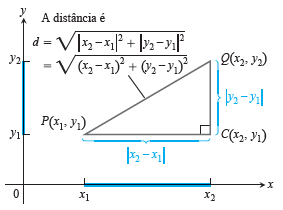
\includegraphics{graficodistancia.png}
    \caption{Descrição da imagem}
    \label{fig:exemplo}
\end{figure}

%
\textbf{Hello World!} Today I am learning \LaTeX. %notice how the command will end at the first non-alphabet charecter such as the . after \LaTeX
\LaTeX{} is a great program for writing math. I can write in line math such as $a^2+b^2=c^2$ %$ tells LaTexX to compile as math
. I can also give equations their own space:
\begin{equation} % Creates an equation environment and is compiled as math
  \gamma^2+\theta^2=\omega^2
\end{equation}
If I do not leave any blank lines \LaTeX{} will continue  this text without making it into a new paragraph.  Notice how there was no indentation in the text after equation (1).
Also notice how even though I hit enter after that sentence and here $\downarrow$
\LaTeX{} formats the sentence without any break.  Also   look  how      it   doesn't     matter          how    many  spaces     I put     between       my    words.
%
For a new essay I can leave a blank space in my code.

\end{document} % This is the end of the document